
\documentclass{beamer} 


\mode<presentation>
{
  \usetheme{Berkeley}
  % or ...

  \setbeamercovered{transparent}
  % or whatever (possibly just delete it)
}

\usepackage{tikz}
\usepackage{graphicx}
\usepackage[english]{babel}
% or whatever

\usepackage[utf8]{inputenc}
% or whatever

\usepackage{times}
\usepackage[T1]{fontenc}
% Or whatever. Note that the encoding and the font should match. If T1
% does not look nice, try deleting the line with the fontenc.


\title[] % (optional, use only with long paper titles)
{Tools for a Reproducible Workflow}


\author[Christensen] % (optional, use only with lots of authors)
{Garret~Christensen\inst{1}}
% - Give the names in the same order as the appear in the paper.
% - Use the \inst{?} command only if the authors have different
%   affiliation.

\institute[Universities of Somewhere and Elsewhere] % (optional, but mostly needed)
{
  \inst{1}%
  UC Berkeley:\\
  Berkeley Initiative for Transparency in the Social Sciences\\
  Berkeley Institute for Data Science\\
  }
% - Use the \inst command only if there are several affiliations.
% - Keep it simple, no one is interested in your street address.

\date[BITSS2016] % (optional, should be abbreviation of conference name)
{BITSS Annual Meeting 2016\\
Slides available online at \url{https://github.com/BITSS/Annual2016}}
% - Either use conference name or its abbreviation.
% - Not really informative to the audience, more for people (including
%   yourself) who are reading the slides online

\subject{Research Transparency}
% This is only inserted into the PDF information catalog. Can be left
% out. 

\pgfdeclareimage[height=2cm]{university-logo}{../Images/BITSSlogo.png}
\logo{\pgfuseimage{university-logo}}


\begin{document}

\begin{frame}
  \titlepage
\end{frame}


%%%%%%%%%%%%%%%%%%%%%%%%%%%%%%%%%%%%%%%%%%%%%%%%%%%%%%%%%%%%%%%%%%%%%%%
%%%%%%%%%%%%%%%%%%%%%%%%%%%%%%%%%%%%%%%%%%%%%%%%%%%%%%%%%%%%%%%%%%%%%

\section {Introduction}
{ % all template changes are local to this group.
    \setbeamertemplate{navigation symbols}{}
    \begin{frame}[plain]
        \begin{tikzpicture}[remember picture,overlay]
            \node[at=(current page.center)] {
                \href{https://www.bitss.org/}{\includegraphics[width=\paperwidth]{../Images/bitsslogo.png}}
            };
        \end{tikzpicture}
     \end{frame}
}


%%%%%%%%%%%%%%%%%%%%%%%%%%%%%%%%%%%%%%%%%%%%%%%%%%%%%%%%%%%%%%%%%%%%%%%%%%%

 \begin{frame}{Reproducibility}
``Reproducibility is just collaboration with people you don't know,
including yourself next week''

---Philip Stark, UC Berkeley Statistics
\end{frame}



%%%%%%%%%%%%%%%%%%%%%%%%%%%%%%%%%%%%%%%%%%%%%%%%%%%%%%%%%%%%%%%%%%
\section{Problems}
\begin{frame}{Problems}
 \begin{itemize}
 \item Data not available
 \item Code not available/unintelligible
 \item Code and data cannot reproduce original results
 \end{itemize}
\end{frame}

 \begin{frame}{Irreproducible Workflow}
 \begin{itemize}
 \item
  Even with the help of the original author (yourself?), you can't get the data to reproduce the published results. Or you just can't find the data to begin with. 
  \item \textit{Journal of Money, Credit, and Banking} Project. \href{http://www.jstor.org/stable/1806061}{(Dewald et al., AER 1986)}
   \item Martin Feldstein on Social Security and private savings, Reinhart and Rogoff on debt and GDP growth.
 \end{itemize} 
 \end{frame}
%%%%%%%%%%%%%%%%%%%%%%%%%%%%%%%%%%%%%%%%%%%%%%%%%%%%%%%%%%%%%%%%%%%%%%%%%%%%%%%%%%%%
\section{Solutions}

\begin{frame}{Reproducibility \& Transparency}
\begin{itemize}
\item \textbf{What are practical tools to implement reproducibility solutions?}
\end{itemize}
\end{frame}

\begin{frame}
 \begin{itemize}
 \item Better Workflow
 \item Dynamic Documents
 \item Version Control
\end{itemize}
\end{frame}
%%%%%%%%%%%%%%%%%%%%%%%%%%%%%%%%%%%%%%%%%%%%%%%%%%%%%%%%%%%%%%%
\subsection{Workflow}
\begin{frame}{Workflow}
\begin{itemize}
\item First, \textit{programming} is key to reproducibility. Working in Excel is not reproducible.
\item See Reinhart and Rogoff ``Growth in a Time of Debt'' controversy: 
\begin{itemize}
	\item
	Original Paper, \href{https://www.aeaweb.org/articles.php?doi=10.1257/aer.100.2.573}{\textit{AER P \& P} 2010}
	\item 
	\href{http://cje.oxfordjournals.org/content/38/2/257}{Herndon et. al (2013)} finding.
	\item \href{http://www.newyorker.com/news/john-cassidy/the-reinhart-and-rogoff-controversy-a-summing-up}{\textit{New Yorker} summary}.
\end{itemize}

\item Random number generation in Excel--set seed with \href{http://www.statisticshowto.com/use-random-number-generator-excel/}{Data Analysis Toolpak}. 
\end{itemize}
\end{frame}

\begin{frame}{Workflow}
\begin{itemize}
\item  If you are using SPSS, use of `syntax' to record all the commands you run is simple. (See \href{http://www.ats.ucla.edu/stat/spss/seminars/spss_syntax/}{UCLA tutorial}.) Similarly in Stata, `commandlog'.

\item Better is to write scripts. R, Stata, SAS, Python, or whatever you please.

\item Open source has some advantages (being free, for one) but you're going to use what everyone in your field uses.
\end{itemize}
\end{frame}

\begin{frame}{Organizing and Recording Workflow}
 Practical suggestions: if you got hit by a bus...
 \begin{itemize}
 \item Making any changes to a file that has been posted/shared means it gets a new name.
 \item Use version commands to ensure others get same results.
 \item Keep a daily research log.
 \item README files.
 \item Long (2008) \textit{The Workflow of Data Analysis Using Stata}
\end{itemize}
\end{frame}


\begin{frame}{Literate Programming}
\begin{itemize}
\item
Second, \textit{literate programming} is key to reproducibility. Write code to be read by a human being, with the code for the computer secondary.
\end{itemize}
\end{frame}

\begin{frame}{Literate Programming}
\begin{quote}
``I believe that the time is ripe for significantly better documentation of programs, and that we can best achieve this by considering programs to be works of literature. Hence, my title: ``Literate Programming.''

Let us change our traditional attitude to the construction of programs: Instead of imagining that our main task is to instruct a computer what to do, let us concentrate rather on explaining to human beings what we want a computer to do.
\end{quote}
(cont.)
\end{frame}

\begin{frame}{Literate Programming}
\begin{quote}
``The practitioner of literate programming can be regarded as an essayist, whose main concern is with exposition and excellence of style. Such an author, with thesaurus in hand, chooses the names of variables carefully and explains what each variable means. He or she strives for a program that is comprehensible because its concepts have been introduced in an order that is best for human understanding, using a mixture of formal and informal methods that reinforce each other.''
\end{quote}
--Donald Knuth \textit{The Computer Journal}, 1984
\href{http://www.literateprogramming.com/index.html}{\beamerbutton{Quotes}}
\href{http://comjnl.oxfordjournals.org/content/27/2/97.full.pdf+html}{\beamerbutton{Original}}
\end{frame}


%%%%%%%%%%%%%%%%%%%%%%%%%%%%%%%%%%%%%%%%%%%%%%%%%%%%%%%%%%%%%%%%%%%%%%%%%%%%


\begin{frame}{Dynamic Documents}
Write your code and your paper in the same file so you won't lose information or make copy and paste mistakes.

\begin{itemize}
\item Include tables by linking to a file, instead of a static image.
\item Include number by linking to a value calculated by an analysis file, instead of a static number typed manually.
\item Automatically update tables and numbers.
\item Produce entire paper with one or two clicks.
\end{itemize} 
\end{frame}

\begin{frame}{Dynamic Documents}
Possible in Python, R, and to a lesser extent, Stata

\begin{itemize}
\item Jupyter---many languages
\item R---use R Studio to manage projects with built-in version control, and R Markdown/knitr for publication-quality dynamic documents.
\item Stata--combine with LaTeX for two click workflow
\item Stata--use `\href{https://github.com/haghish/MarkDoc}{markdoc}' or \href{http://www.stata.com/meeting/oceania16/slides/rising-oceania16.pdf}{other} ado for some dynamic ability.
\end{itemize} 
\end{frame}

 
 { % all template changes are local to this group.
    \setbeamertemplate{navigation symbols}{}
    \begin{frame}[plain, label=AEAreg]
         \begin{tikzpicture}[remember picture,overlay]
            \node[at=(current page.center)] {
                
\includegraphics[width=\paperwidth]{../Images/RStudio-Logo-Blue-Gradient.png}
            };
        \end{tikzpicture}
     \end{frame}
}

{ % all template changes are local to this group.
    \setbeamertemplate{navigation symbols}{}
    \begin{frame}[plain, label=AEAreg]
         \begin{tikzpicture}[remember picture,overlay]
            \node[at=(current page.center)] {
                
\includegraphics[height=\paperheight]{../Images/jupyter.png}
            };
        \end{tikzpicture}
     \end{frame}
}


\begin{frame}{Examples}
\begin{itemize}
\item
Stata Example

\item
R Studio Example

\end{itemize}
\end{frame}
%%%%%%%%%%%%%%%%%%%%%%%%%%%%%%%%%%%%%%%%%%%%%%%%%%%%%%%%%%%%%%%%%%%%
%%%%%%%%%%%%%%%%%%%%%%%%%%%%%%%%%%%%%%%%%%%%%%%%%%%%%%%%%%%%%%%%%%%%%
%%%%%%%%%%%%%%%%%%%%%%%%%%%%%%%%%%%%%%%%%%%%%%%%%%%%%%%%%%%%%%%%%%%%%


\subsection{Version Control}
 { % all template changes are local to this group.
    \setbeamertemplate{navigation symbols}{}
    \begin{frame}[plain, label=AEAreg]
         \begin{tikzpicture}[remember picture,overlay]
            \node[at=(current page.center)] {
                
\includegraphics[height=\paperheight]{../Images/github-logo-transparent.JPG}
            };
        \end{tikzpicture}
     \end{frame}
}

%%%%%%%%%%%%%%%%%%%%%%%%%%%%%%%%%%%%%%%%%%%%%%%%%%%%%%%%%%%%%%%%%%%%%

\begin{frame}{Version Control}
\begin{itemize}
\item
Using version control (AKA revision control) can help to make your work more reproducible.

\item
What is version control?

\begin{quote}
Version control is a system that records changes to a file or set of files over time so that you can recall specific versions later. For the examples in this book you will use software source code as the files being version controlled, though in reality you can do this with nearly any type of file on a computer.
\end{quote}
--Git, \href{https://git-scm.com/book/en/v2/Getting-Started-About-Version-Control}{About Version Control}

%\item Distributed Version Control Systems (DCVS) let multiple users control the same files in this manner.
\end{itemize}
\end{frame}
%%%%%%%%%%%%%%%%%%%%%%%%%%%%%%%%%%%%%%%%%%%%%%%%%%%%%%%
\begin{frame}{Version Control}
With version control you can:
\begin{itemize}
\item Collaborate 
\item Track who made every change
\item Easily switch between versions of files
\item Compare versions of files
\item Backup
\item Work with the same files on different machines
\item Experiment with a new version of code without breaking things
\end{itemize}
\href{http://stackoverflow.com/questions/1408450/why-should-i-use-version-control}{\beamerbutton{Link1}}
\href{http://tex.stackexchange.com/questions/1118/what-are-the-advantages-of-using-version-control-git-cvs-etc-in-latex-documen}{\beamerbutton{Link2}}
\href{http://stackoverflow.com/questions/1408450/why-should-i-use-version-control}{\beamerbutton{Link3}}
\end{frame}
%%%%%%%%%%%%%%%%%%%%%%%%%%%%%%%%%%%%%%%%%%%

\begin{frame}{Version Control}
Places you're already using version control without knowing it:
\end{frame}
%%%%%%%%%%%%%%%%%%%%%%%%%%%%%%%%%%%%%%%


{ % all template changes are local to this group.
    \setbeamertemplate{navigation symbols}{}
    \begin{frame}[plain]
        \begin{tikzpicture}[remember picture,overlay]
            \node[at=(current page.center)] {
                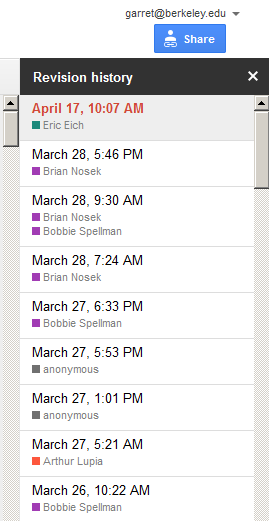
\includegraphics[height=\paperheight]{../Images/googledocs.PNG}
            };
        \end{tikzpicture}
     \end{frame}

 \setbeamertemplate{navigation symbols}{}
    \begin{frame}[plain]
        \begin{tikzpicture}[remember picture,overlay]
            \node[at=(current page.center)] {
                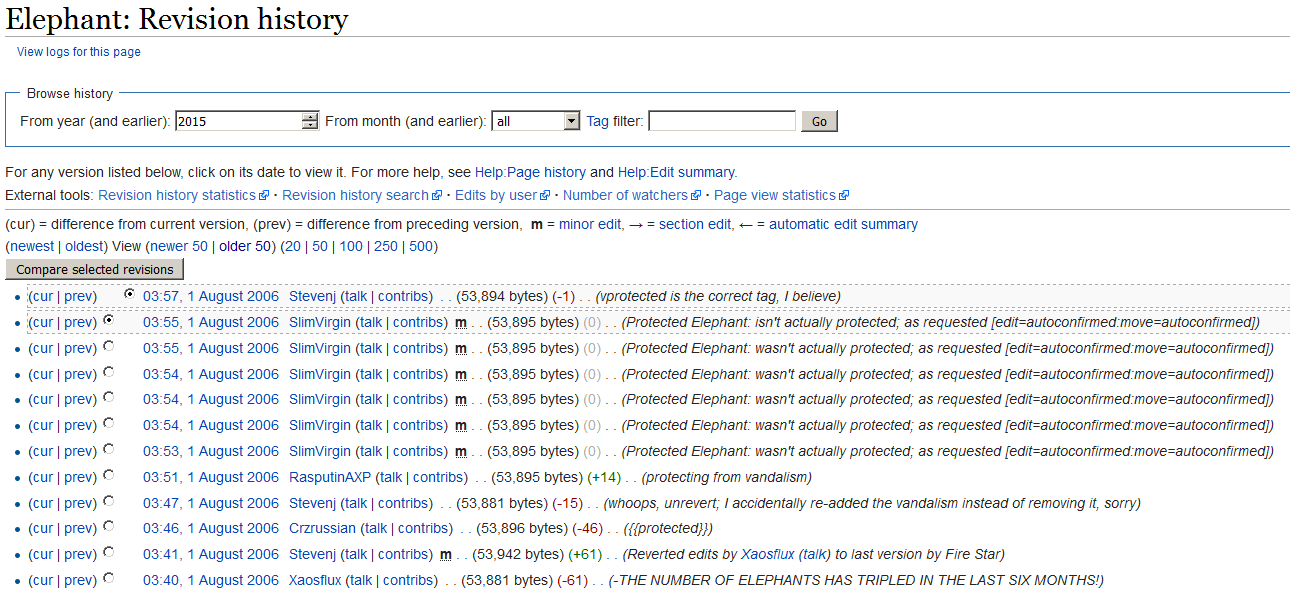
\includegraphics[width=\paperwidth]{../Images/elephantswiki.PNG}
            };
        \end{tikzpicture}
     \end{frame}
}
\begin{frame}{Version Control}
Places you're already using version control without knowing it:
\begin{itemize}
	\item
	Google Docs
	\item
	Wikipedia
	\item
	Every piece of software you use.
\end{itemize}
\end{frame}

%%%%%%%%%%%%%%%%%%%%%%%%
\begin{frame}{Version Control}
Isn't this just a complicated version of the ``date and initial'' method?
\begin{itemize}
\item regressions2015.08.24.do
\item regressions2015.08.25.do
\item regressions2015.08.25GC.do
\item Hassle
\item Confusion \href{http://www.phdcomics.com/comics/archive.php?comicid=1531}{\beamergotobutton{Comic}}
\end{itemize}
\end{frame}

\begin{frame}{Version Control}
\begin{quote}Here is a good rule of thumb: If you are trying to solve a problem, and there are multi-billion dollar  firms  whose  entire  business  model  depends  on  solving  the  same  problem,  and  there  are whole courses at your university devoted to how to solve that problem, you might want to figure out what the experts do and see if you can’t learn something from it.

...

Not one piece of commercial software you have on your PC, your phone, your tablet,
your car, or any other modern computing device was written with the “date and initial” method.
\end{quote}
--Matthew Gentzkow and Jesse M. Shapiro ``\href{http://web.stanford.edu/~gentzkow/research/CodeAndData.pdf}{Code and Data for the Social Sciences: A Practitioner's Guide}''
\end{frame}


{ % all template changes are local to this group.
    \setbeamertemplate{navigation symbols}{}
     
     \begin{frame}[plain]
         \begin{tikzpicture}[remember picture,overlay]
            \node[at=(current page.center)] {
               \href{https://xkcd.com/1597/}{
\includegraphics[height=\paperheight]{../Images/git.png}}
            };
        \end{tikzpicture}
     \end{frame}

    \begin{frame}[plain]
        \begin{tikzpicture}[remember picture,overlay]
            \node[at=(current page.center)] {
                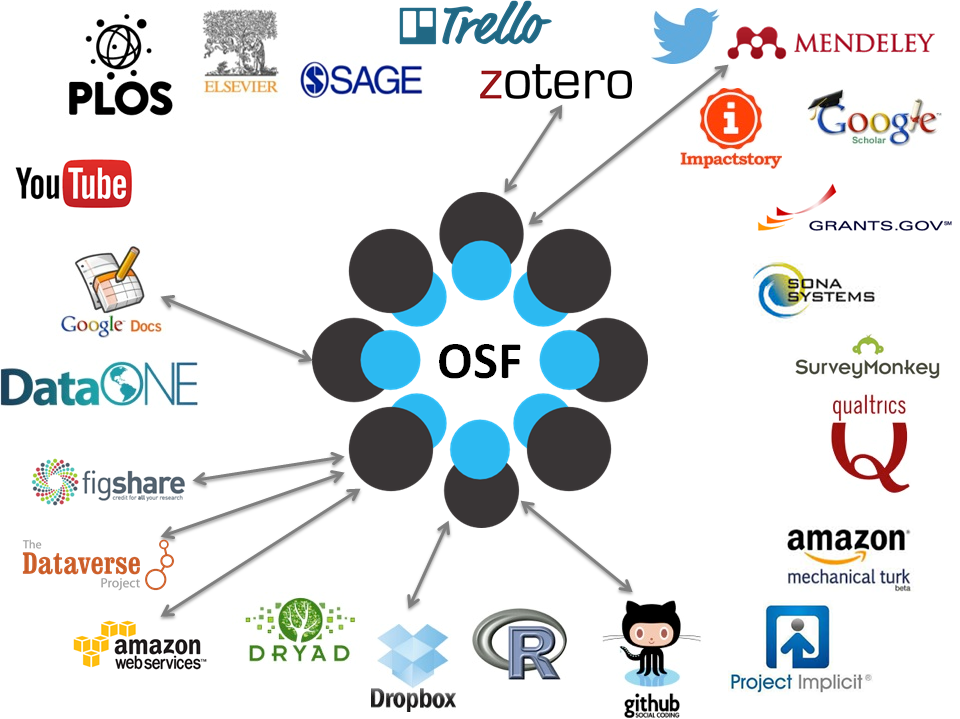
\includegraphics[height=\paperheight]{../Images/OSFnow.PNG}
            };
        \end{tikzpicture}
     \end{frame}
 
    \begin{frame}[plain]
        \begin{tikzpicture}[remember picture,overlay]
            \node[at=(current page.center)] {
                
\includegraphics[height=\paperheight]{../Images/OSFsoon.PNG}
            };
        \end{tikzpicture}
     \end{frame}
}
%%%%%%%%%%%%%%%
\begin{frame}{Examples}
GitHub and OSF Examples:
\begin{itemize}
\item
Slides for this workshop on Github.com
\item \url{http://www.github.com/bitss/annual2016}
\item
Slides also available on the Open Science Framework
 \item \url{https://osf.io/t3ttm/}
\end{itemize}
\end{frame}
%%%%%%%%%%%%%%%%%%%%%%%%%%%%%%%%%%%%%%%%%%%%%%%%%%%%%%%%%%%%%%%%%%%%%



\section{Conclusion}
\begin{frame}{Conclusion}
Simple tools exist to help you transparently and reproducibly take your research from beginning to end. 
\begin {itemize}

\item Version Control
\item Open Science Framework
\item Dynamic Documents
\end{itemize} 

Learn more: 
\begin{itemize}
\item
Read my \href{http://github.com/garretchristensen/manual}{\textit{Manual of Best Practices in Transparent Social Science Research}} on GitHub.

\item Work through my demos.\href{https://github.com/BITSS/ICPSR2016}{\beamergotobutton{Link}}
\item Software Carpentry's tutorials \href{http://www.software-carpentry.org/lessons}{\beamergotobutton{Link}}
\end{itemize}
\end{frame}

\end{document}

